\chapter{Retrieval-Augmented Generation (RAG)}
\section{Retrieval-Augmented Generation (RAG)}

Large Language Models (LLMs) possess an impressive amount of general knowledge acquired during pretraining. However, they cannot answer questions about information that was never included in their training data.

Consider the following question:

\begin{quote}
\textbf{``What is the vacation policy of my company?''}
\end{quote}

Although models such as ChatGPT have extensive general knowledge, they have never seen a company's private documents unless those documents are explicitly provided during inference. Consequently, the model can only answer using the knowledge stored during pretraining.
\subsection*{Parametric Memory}

During pretraining, an LLM learns statistical patterns from massive collections of text. This knowledge is encoded inside the model parameters (weights), which collectively form the model's \textbf{parametric memory}.
\begin{figure}[H]
\centering
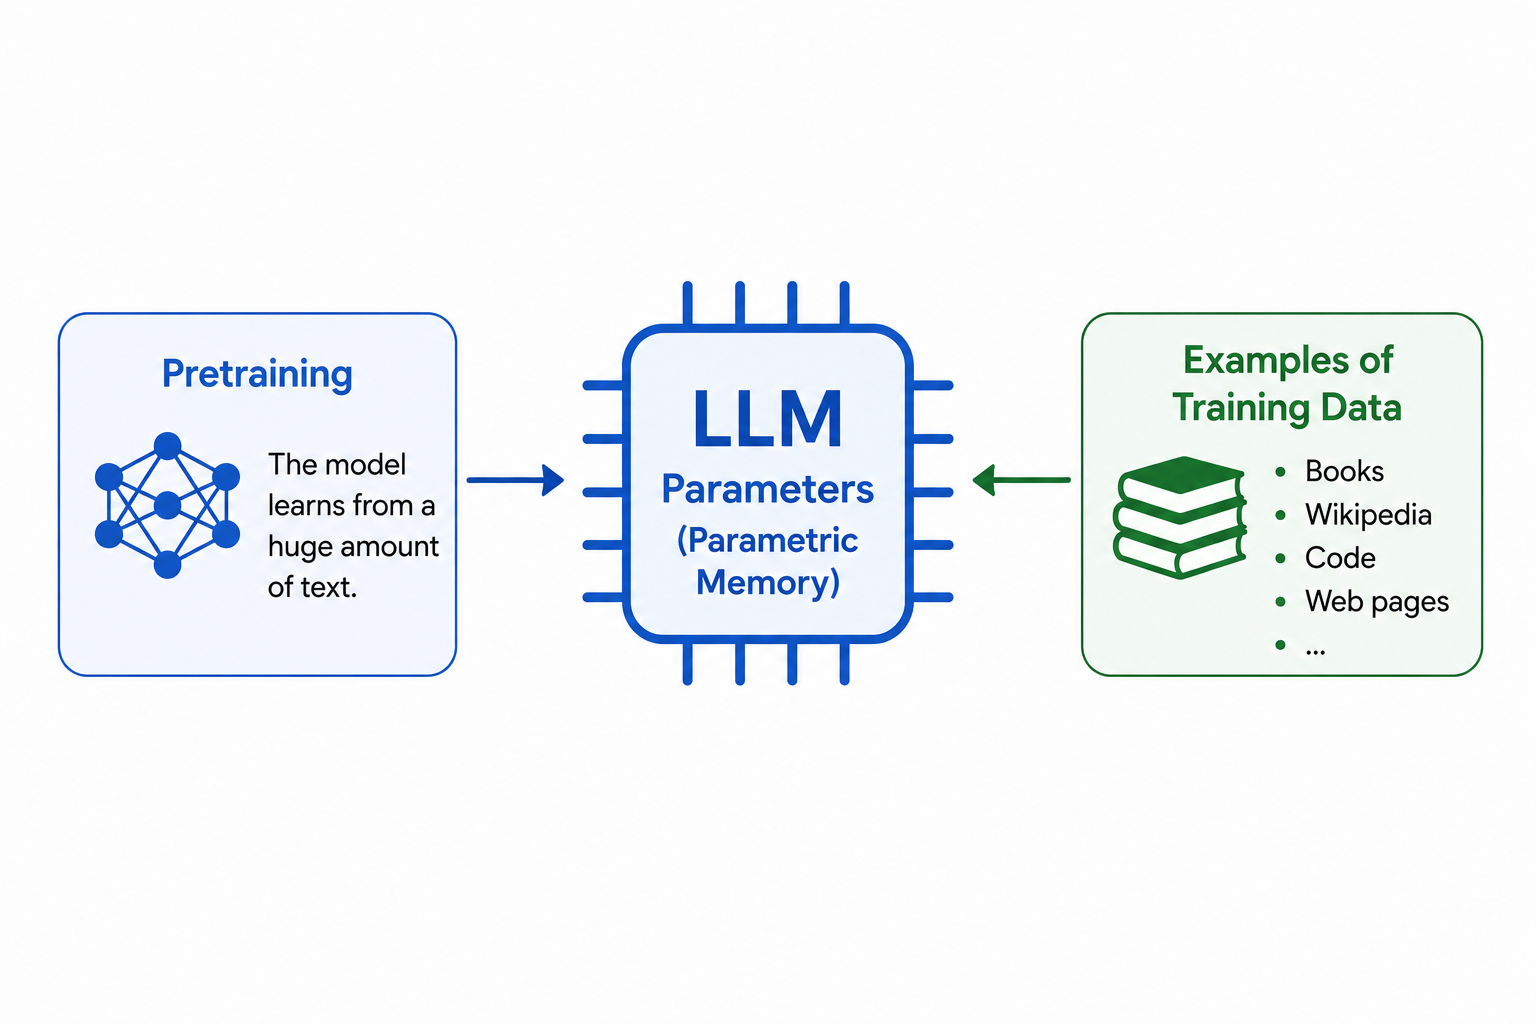
\includegraphics[width=0.85\textwidth]{figures/13-1 figure.png}
\caption{Knowledge stored in the parameters of a pretrained language model (parametric memory).}
\end{figure}
Because this knowledge is permanently embedded in the model parameters, the model can answer a wide variety of general questions without consulting any external source.
The main advantages of parametric memory are:

\begin{itemize}
\item Fast inference since no external retrieval is required.
\item No dependency on an external database.
\item Extensive general-world knowledge acquired during pretraining.
\end{itemize}
\subsection*{Limitations}

Despite its strengths, parametric memory has several important limitations:

\begin{itemize}
\item Knowledge becomes outdated after training.
\item Private documents cannot be accessed.
\item Newly available information cannot be incorporated instantly.
\item Updating the knowledge requires retraining or fine-tuning the model.
\end{itemize}
\subsection*{The Main Idea Behind RAG}

Retrieval-Augmented Generation (RAG) addresses this limitation by retrieving only the documents that are relevant to the user's question instead of permanently storing the information inside the model.

Rather than modifying the model's parameters, RAG supplies the required knowledge dynamically during inference.

\begin{figure}[H]
\centering
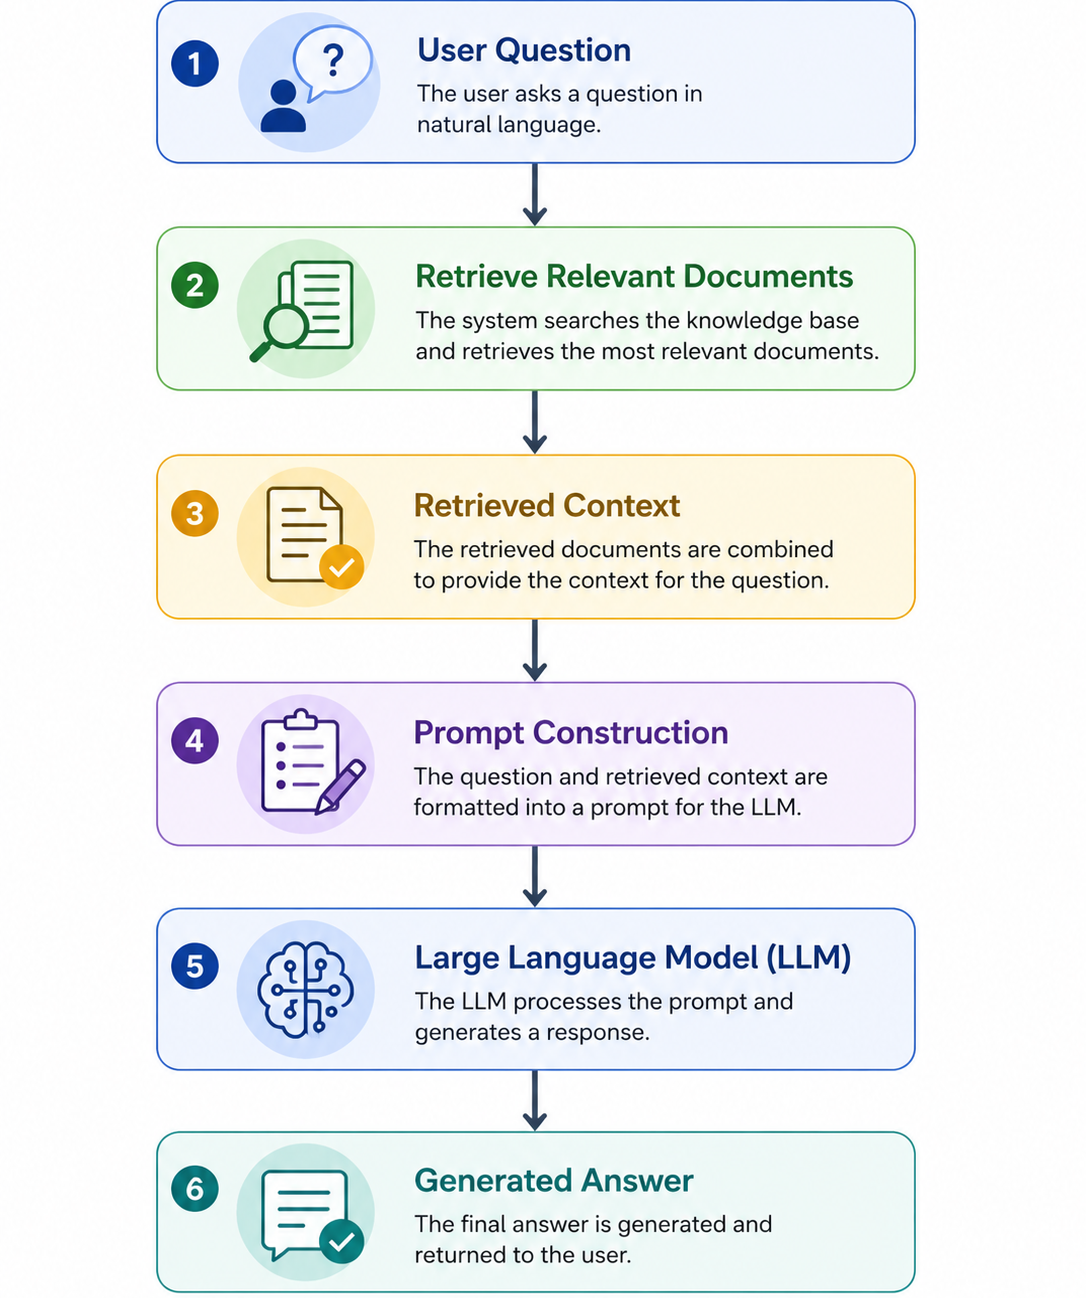
\includegraphics[width=0.85\textwidth]{figures/13-55 figure.png}
\end{figure}

The retrieved documents are appended to the prompt and provided to the language model, enabling it to generate answers based on external information.

Importantly, RAG does not require retrieved information to be permanently encoded in the model's parameters. Instead, the model reads the retrieved context during inference and uses it to produce the final response.
\paragraph{Key Idea}

RAG provides knowledge \textbf{when it is needed} instead of storing that knowledge permanently inside the model parameters.
\begin{figure}[H]
\centering
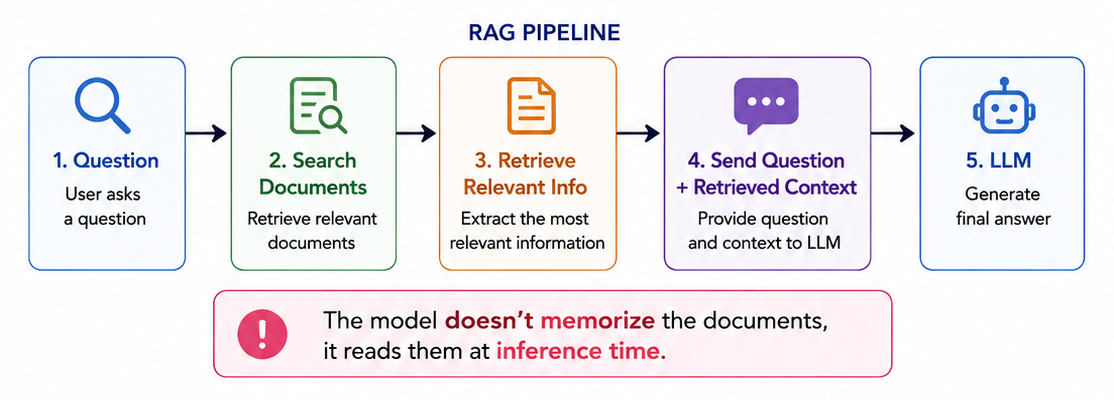
\includegraphics[width=0.85\textwidth]{figures/13-22 figure.png}
\end{figure}
Consequently, the language model remains unchanged while still benefiting from up-to-date or private information stored in external knowledge sources.
\subsection*{Example}

Assume that the company's employee handbook contains the following information.
\begin{figure}[H]
\centering
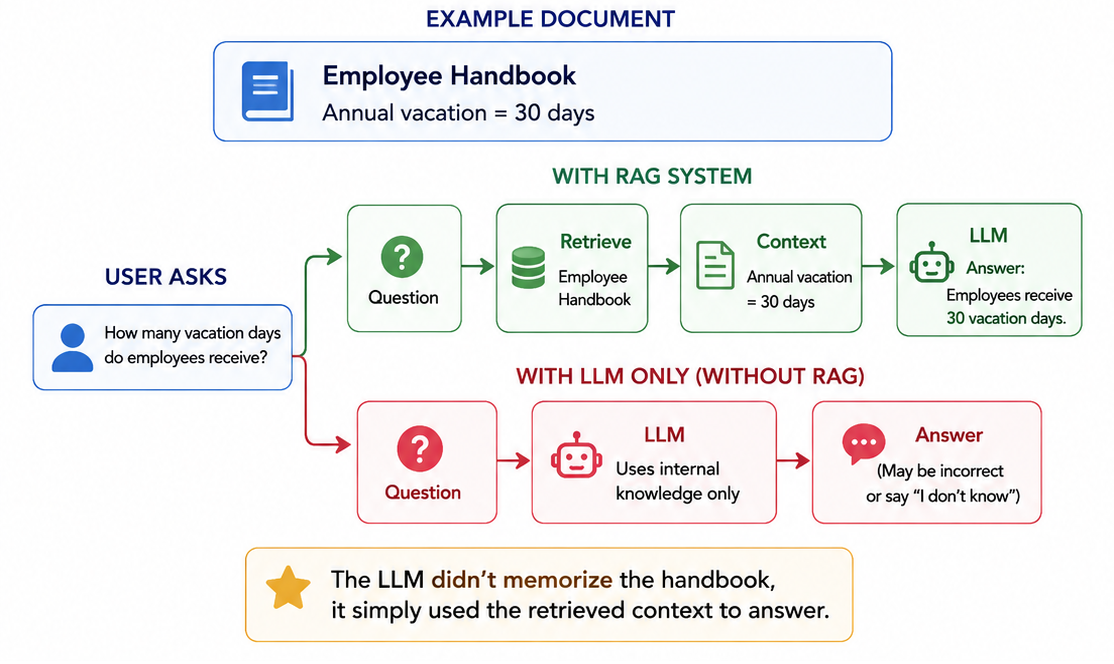
\includegraphics[width=0.85\textwidth]{figures/13-2 figure.png}
\end{figure}

Suppose the user asks:

\begin{quote}
\textbf{``How many vacation days do employees receive?''}
\end{quote}

The RAG system first retrieves the employee handbook because it contains information related to the question. The retrieved document indicates that employees receive \textbf{30 vacation days annually}. This information is then appended to the prompt before being sent to the language model.

Finally, the LLM generates the following answer:

\begin{quote}
\textbf{Employees receive 30 vacation days annually.}
\end{quote}

Notice that the model did not memorize the employee handbook. Instead, it simply used the retrieved context at inference time to generate an accurate response.


\section{Parametric vs. Non-Parametric Memory}

As discussed previously, the language model did not memorize the employee handbook. Instead, it generated the answer by using the retrieved document during inference.

This highlights an important distinction between two types of knowledge used by modern LLMs: \textbf{parametric memory} and \textbf{non-parametric memory}.

\subsection*{Parametric Memory}

Parametric memory refers to the knowledge permanently stored inside the model's parameters (weights) during pretraining.

Examples include:

\begin{itemize}
    \item General world knowledge.
    \item Grammar and language understanding.
    \item Reasoning abilities.
    \item Coding patterns.
\end{itemize}

\subsection*{Non-Parametric Memory}

Non-parametric memory refers to knowledge stored outside the language model. Instead of being encoded in the model's parameters, the information is retrieved from external sources whenever it is needed.

Examples include:

\begin{itemize}
    \item PDF documents.
    \item Databases.
    \item Company documents.
    \item Wikis and knowledge bases.
    \item External APIs.
\end{itemize}

Retrieval-Augmented Generation (RAG) combines these two sources of knowledge by allowing the language model to retrieve relevant external information before generating a response.

\begin{figure}[H]
\centering
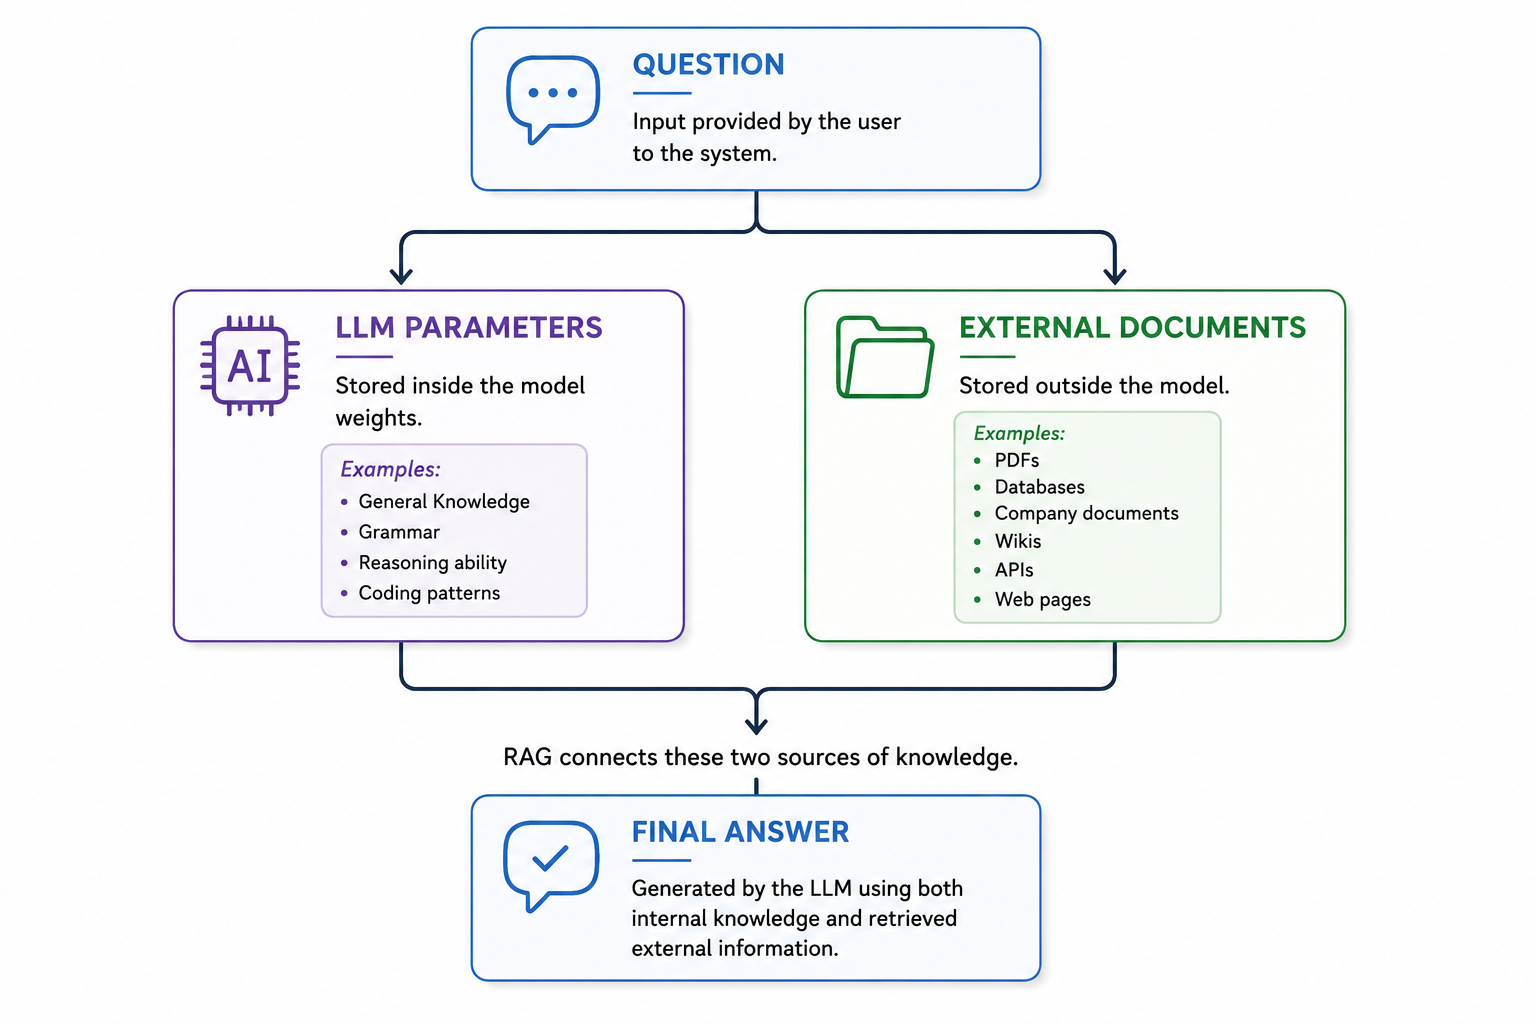
\includegraphics[width=0.85\textwidth]{figures/13-3 figure.png}
\caption{RAG combines parametric memory with non-parametric memory to generate more accurate responses.}
\label{fig:parametric_vs_nonparametric}
\end{figure}

This combination explains why RAG has become widely adopted in real-world applications. Organizations rarely require a model that knows everything. Instead, they need a model capable of accessing and reasoning over their own proprietary data.

Typical examples include:

\begin{itemize}
    \item Hospital records.
    \item Legal documents.
    \item Financial reports.
    \item Product manuals.
    \item Customer support knowledge bases.
\end{itemize}

By retrieving information from these external sources, RAG enables an LLM to answer domain-specific questions without requiring retraining.

\subsection*{Document Chunking}

Suppose we have a PDF document containing 200 pages.

A natural question is:

\begin{center}
\textbf{Can we generate a single embedding for the entire document?}
\end{center}

Technically, the answer is \textbf{yes}. However, in practice, this approach produces poor retrieval performance.

Consider the following document:

\begin{itemize}
    \item Page 5: Vacation Policy.
    \item Page 78: Medical Insurance.
    \item Page 150: Travel Expenses.
\end{itemize}

If a user asks:

\begin{quote}
\textbf{"What is the vacation policy?"}
\end{quote}

the embedding represents the semantic content of all 200 pages simultaneously. Consequently, information about the vacation policy becomes mixed with unrelated topics such as insurance and travel expenses.

As a result, the retriever cannot accurately locate the specific information required to answer the user's question.

Embedding an entire document into a single vector therefore reduces retrieval accuracy because multiple topics are compressed into one representation.

The standard solution is \textbf{document chunking}. Instead of embedding the entire document, the document is divided into smaller chunks, and a separate embedding is generated for each chunk.

\begin{figure}[H]
\centering
\begin{tikzpicture}[
node distance=0.9cm,
every node/.style={font=\small},
box/.style={
draw=blue!70,
fill=blue!10,
rounded corners=4pt,
minimum width=2.9cm,
minimum height=0.95cm,
align=center
},
arrow/.style={
-{Latex[length=2.8mm]},
thick,
blue!70
}
]

\node[box] (pdf) {PDF\\Document};

\node[box,right=of pdf] (chunk)
{Split into\\Chunks};

\node[box,right=of chunk] (embed)
{Generate\\Embeddings};

\node[box,right=of embed] (db)
{Vector\\Database};

\draw[arrow] (pdf) -- (chunk);
\draw[arrow] (chunk) -- (embed);
\draw[arrow] (embed) -- (db);

\end{tikzpicture}
\label{fig:chunk_pipeline}
\end{figure}
Retrieval is therefore performed on individual chunks rather than on the entire document.

\subsection*{Choosing the Chunk Size}

The size of each chunk has a significant impact on retrieval quality.

\begin{itemize}
    \item \textbf{Small chunks} provide more precise retrieval but may omit important surrounding context.
    \item \textbf{Large chunks} preserve more context but may include irrelevant information and increase the number of input tokens sent to the language model.
\end{itemize}

The objective is to find a balance between retrieval precision and contextual completeness.

\begin{figure}[H]
\centering
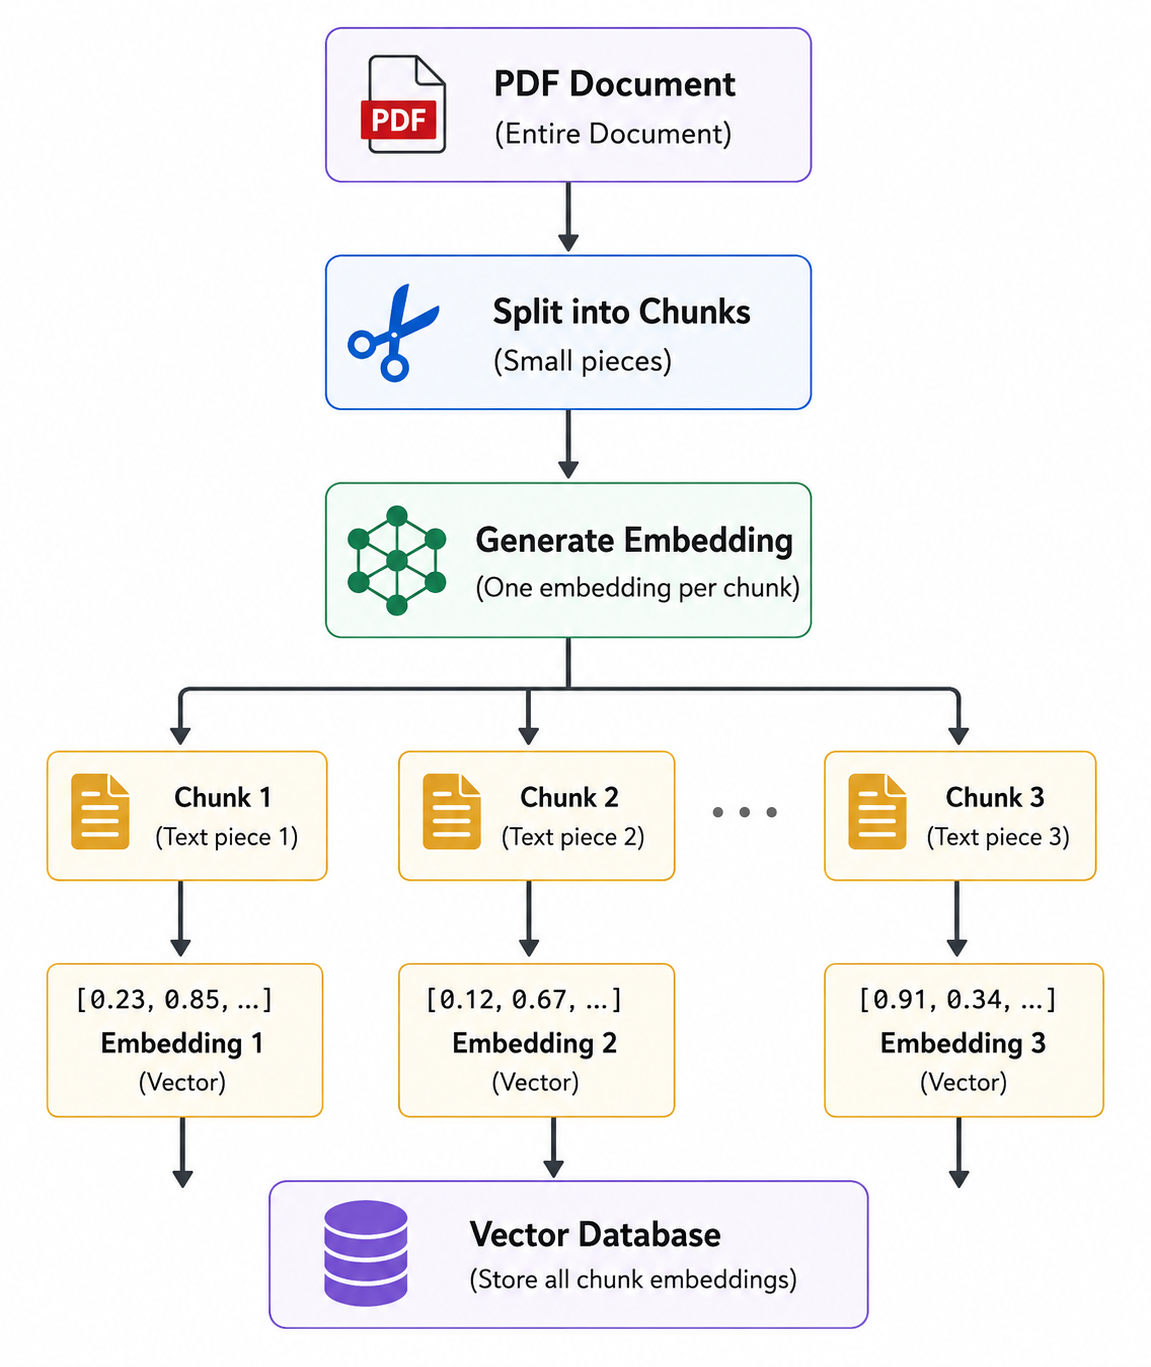
\includegraphics[width=0.85\textwidth]{figures/13-33 figure.png}
\caption{Effect of chunk size on retrieval quality and contextual information.}
\label{fig:chunk_size}
\end{figure}





\subsection*{Chunk Overlap}

In many documents, important information spans multiple chunks. A sentence or concept may begin near the end of one chunk and continue into the next. Without special handling, the meaning can be lost because the information is split across chunk boundaries.

To preserve context, consecutive chunks share a small portion of text. This technique is called \textbf{chunk overlap}. A common starting point is an overlap of approximately 10\% to 20\%, although the optimal overlap depends on the document structure, tokenizer, chunk size, retrieval method, embedding model, and application.

\begin{figure}[H]
\centering
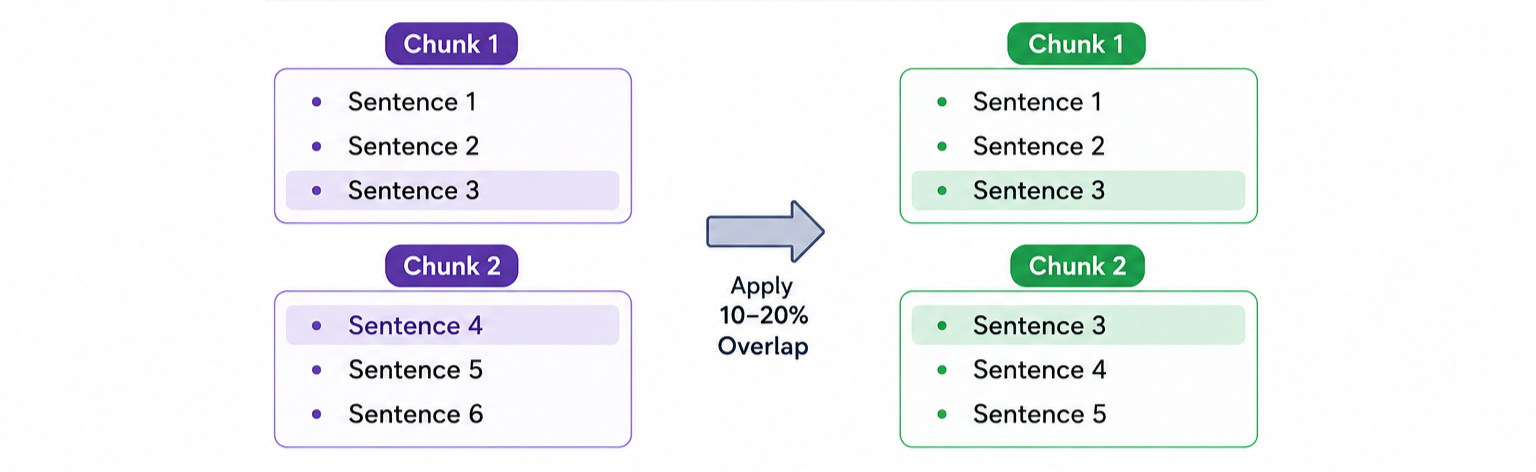
\includegraphics[width=0.85\textwidth]{figures/13-4 figure.png}
\caption{Chunk overlap preserves contextual information across chunk boundaries.}
\label{fig:chunk_overlap}
\end{figure}

For example, suppose a concept begins in Sentence 3 and finishes in Sentence 4. Without overlap, these sentences may be placed in different chunks, making it difficult for the retriever to understand the complete idea.

With chunk overlap, Sentence 3 appears in both chunks, allowing the semantic relationship between the two chunks to be preserved.

Example starting values are:

\begin{itemize}
    \item 10\%
    \item 15\%
    \item 20\%
\end{itemize}

Choosing the overlap size involves a trade-off:

\begin{itemize}
    \item Too much overlap duplicates information and increases storage and computation.
    \item Too little overlap may break the context between consecutive chunks.
\end{itemize}
\subsection*{Types of Chunking}

There is no single strategy for splitting documents into chunks. Different applications require different chunking methods. The three most commonly used approaches are described below.

\subsubsection*{1. Fixed-Size Chunking}

Fixed-size chunking divides a document into chunks containing a predefined number of tokens (for example, 500 tokens per chunk).

This approach is simple, fast, and easy to implement. However, it ignores the natural structure of the document and may split paragraphs or sentences in the middle.

\subsubsection*{2. Recursive Chunking}

Recursive chunking is a widely used practical strategy in modern RAG systems.

Instead of splitting the document after a fixed number of tokens, recursive chunking attempts to preserve the natural structure of the document.

The algorithm begins with the largest structural units, such as headings. If a section exceeds the desired chunk size, it is recursively divided into smaller units such as paragraphs. If a paragraph is still too large, it is further divided into sentences.

For example, suppose the maximum chunk size is 500 tokens and Chapter 1 contains 1200 tokens. Rather than cutting the text arbitrarily, the algorithm first splits the chapter into paragraphs. If one paragraph remains too large, it is divided into sentences until each chunk satisfies the size constraint.

This strategy preserves semantic coherence while respecting the maximum chunk size.
\begin{figure}[H]
\centering
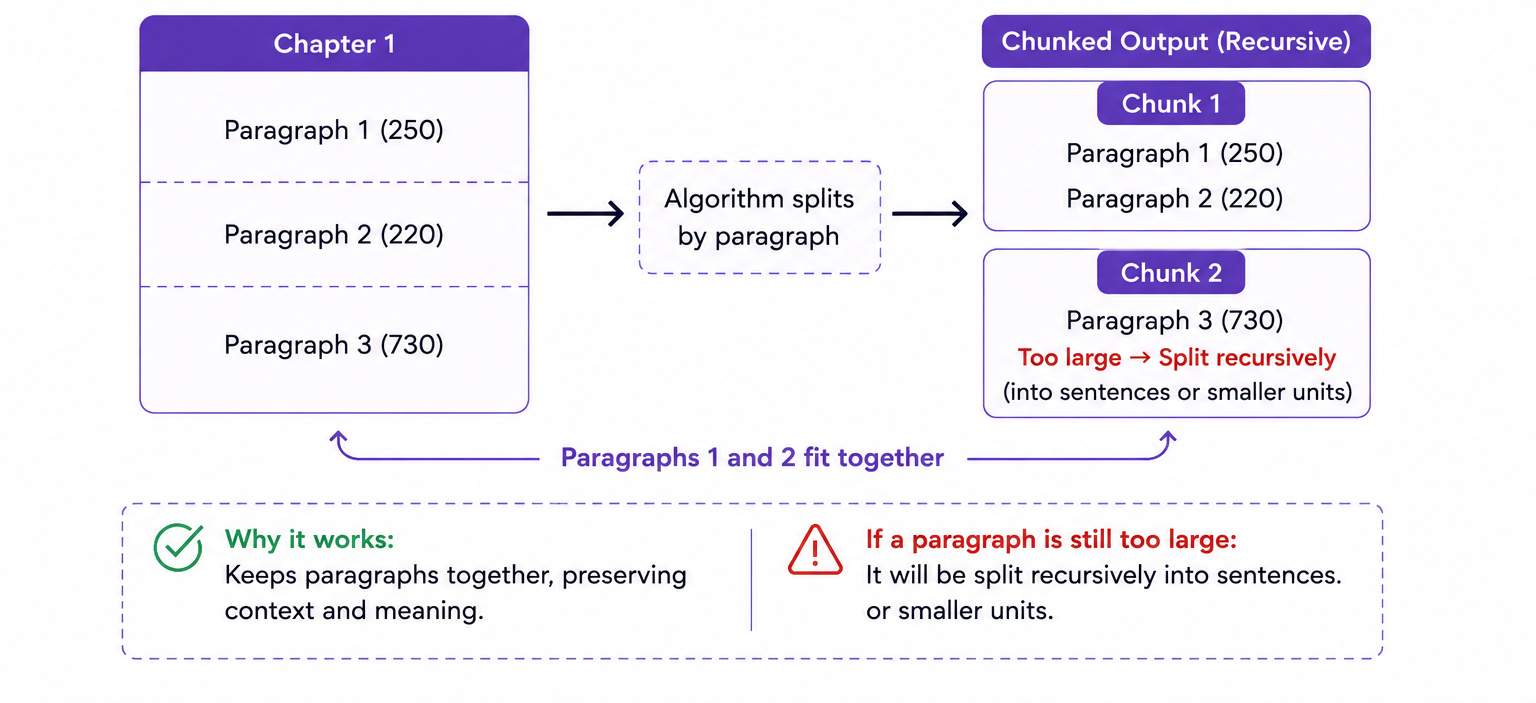
\includegraphics[width=0.85\textwidth]{figures/13-5 figure.png}
\label{fig:recursive_chunking}
\end{figure}
\subsubsection*{3. Semantic Chunking}

Semantic chunking divides a document according to its meaning rather than its length.

Instead of counting tokens, the algorithm measures the semantic similarity between consecutive sentences and creates a new chunk whenever the topic changes.

Although semantic chunking usually produces more meaningful chunks, it is computationally more expensive than fixed-size or recursive chunking.
\subsection*{Metadata}

Each chunk stored in the vector database contains two components:

\begin{itemize}
    \item The chunk text.
    \item Associated metadata.
\end{itemize}

Typical metadata includes:

\begin{itemize}
    \item Document name.
    \item Page number.
    \item Section title.
    \item Author.
    \item Creation date.
\end{itemize}

Metadata enables filtered retrieval. For example, a system may search only human resources documents or retrieve information from a specific document or page.

\begin{figure}[H]
\centering
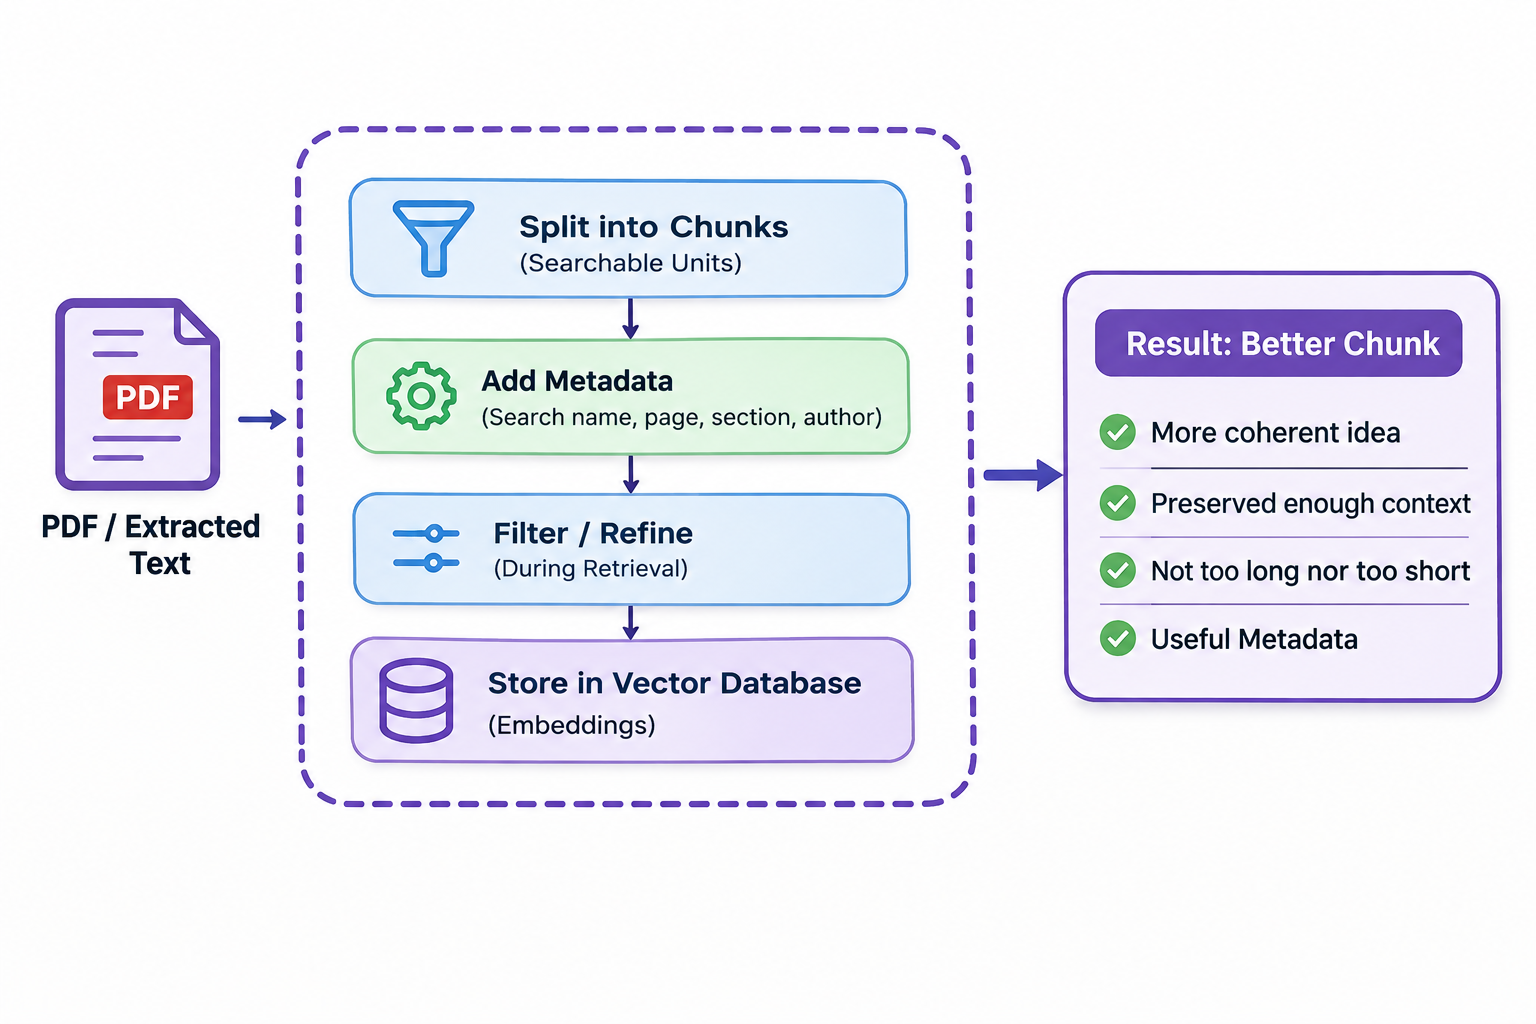
\includegraphics[width=0.85\textwidth]{figures/13-6 figure.png}
\caption{Each chunk is stored together with descriptive metadata.}
\label{fig:metadata}
\end{figure}
\section{Embedding Models}

An embedding model converts text into a numerical vector that captures its semantic meaning.

\begin{center}
\textbf{Text $\rightarrow$ Embedding Model $\rightarrow$ Vector}
\end{center}

Unlike a generative Large Language Model, an embedding model does not generate text. Its sole purpose is to transform textual information into dense vector representations, where semantically similar texts are located close to one another in the embedding space.

A high-quality embedding model should assign similar vectors to texts that express the same meaning, even if they use different words.

For example,

\begin{quote}
``What is Artificial Intelligence?''
\end{quote}

and

\begin{quote}
``Explain Artificial Intelligence.''
\end{quote}

should produce vectors that are very close together because they convey nearly identical semantic content.

Several embedding models are widely used in production systems, including:

\begin{itemize}
    \item BGE-M3
    \item Multilingual-e5-large
    \item Voyage-3
    \item OpenAI \texttt{text-embedding-3-large}
    \item Jina Embeddings v3
\end{itemize}


\section{Vector Database}

A \textbf{vector database} is a specialized database designed to store vector embeddings and perform efficient similarity search.

Unlike traditional relational databases (SQL), which are optimized for exact matching, filtering, and joins, vector databases are optimized for finding vectors that are semantically similar to a query vector.

Each document chunk is stored as a record containing:

\begin{itemize}
    \item A unique identifier (ID).
    \item The embedding vector.
    \item The original text.
    \item Associated metadata (e.g., page number, document name, author, etc.).
\end{itemize}
\section{Popular Vector Databases}

Several vector databases are widely used in modern Retrieval-Augmented Generation (RAG) systems, including:

\begin{itemize}
    \item FAISS (Facebook AI Similarity Search)
    \item Qdrant
    \item Chroma
    \item Pinecone
\end{itemize}

The typical retrieval pipeline is illustrated below:

\begin{center}
\textbf{User Query $\rightarrow$ Embedding Model $\rightarrow$ Query Vector $\rightarrow$ Vector Database $\rightarrow$ Top-$k$ Chunks $\rightarrow$ LLM}
\end{center}

The vector database returns the chunks whose embeddings are the most similar to the query embedding.
\section{Retrieval Methods}

Modern RAG systems generally use two retrieval strategies: \textbf{dense retrieval} and \textbf{sparse retrieval}.

\subsection*{1. Dense Retrieval}

Dense retrieval represents both documents and queries using embeddings. Similarity is then computed in the embedding space.

Its main advantages are:

\begin{itemize}
    \item Captures semantic meaning.
    \item Handles synonyms and paraphrases.
    \item Works well even when different words express the same idea.
\end{itemize}

However, dense retrieval may struggle with exact terms such as:

\begin{itemize}
    \item Product IDs.
    \item Error codes.
    \item Person names.
    \item File names.
    \item Rare words.
    \item Exact phrases.
\end{itemize}

For example, given the query

\begin{quote}
\texttt{ERR-9238-X}
\end{quote}

a dense retriever may fail to retrieve the correct document because it focuses on semantic similarity rather than exact keyword matching.

\subsection*{2. Sparse Retrieval (BM25)}

Sparse retrieval is based on keyword matching instead of semantic similarity. The most widely used sparse retrieval algorithm is \textbf{BM25}.

Its main characteristics are:

\begin{itemize}
    \item Uses keyword matching.
    \item Retrieves exact matches.
    \item Performs well for IDs, codes, names, and numbers.
\end{itemize}

For example,

\begin{quote}
\texttt{ERR-9238-X}
\end{quote}

directly retrieves documents containing the exact identifier.

Sparse retrieval is particularly effective for:

\begin{itemize}
    \item IDs.
    \item Product codes.
    \item Person names.
    \item Exact technical terms.
\end{itemize}
\section{Hybrid Search}

Dense retrieval and sparse retrieval complement each other because they excel at different tasks.

Consider the following query:

\begin{quote}
\textbf{``Error ERR-9238-X in the payment system''}
\end{quote}

Dense retrieval captures the semantic concepts:

\begin{itemize}
    \item Payment.
    \item System.
    \item Error.
\end{itemize}

Sparse retrieval identifies the exact keyword:

\begin{itemize}
    \item ERR-9238-X.
\end{itemize}

Instead of selecting only one retrieval strategy, modern RAG systems often combine both approaches. This technique is known as \textbf{Hybrid Search}.

\begin{figure}[H]
\centering
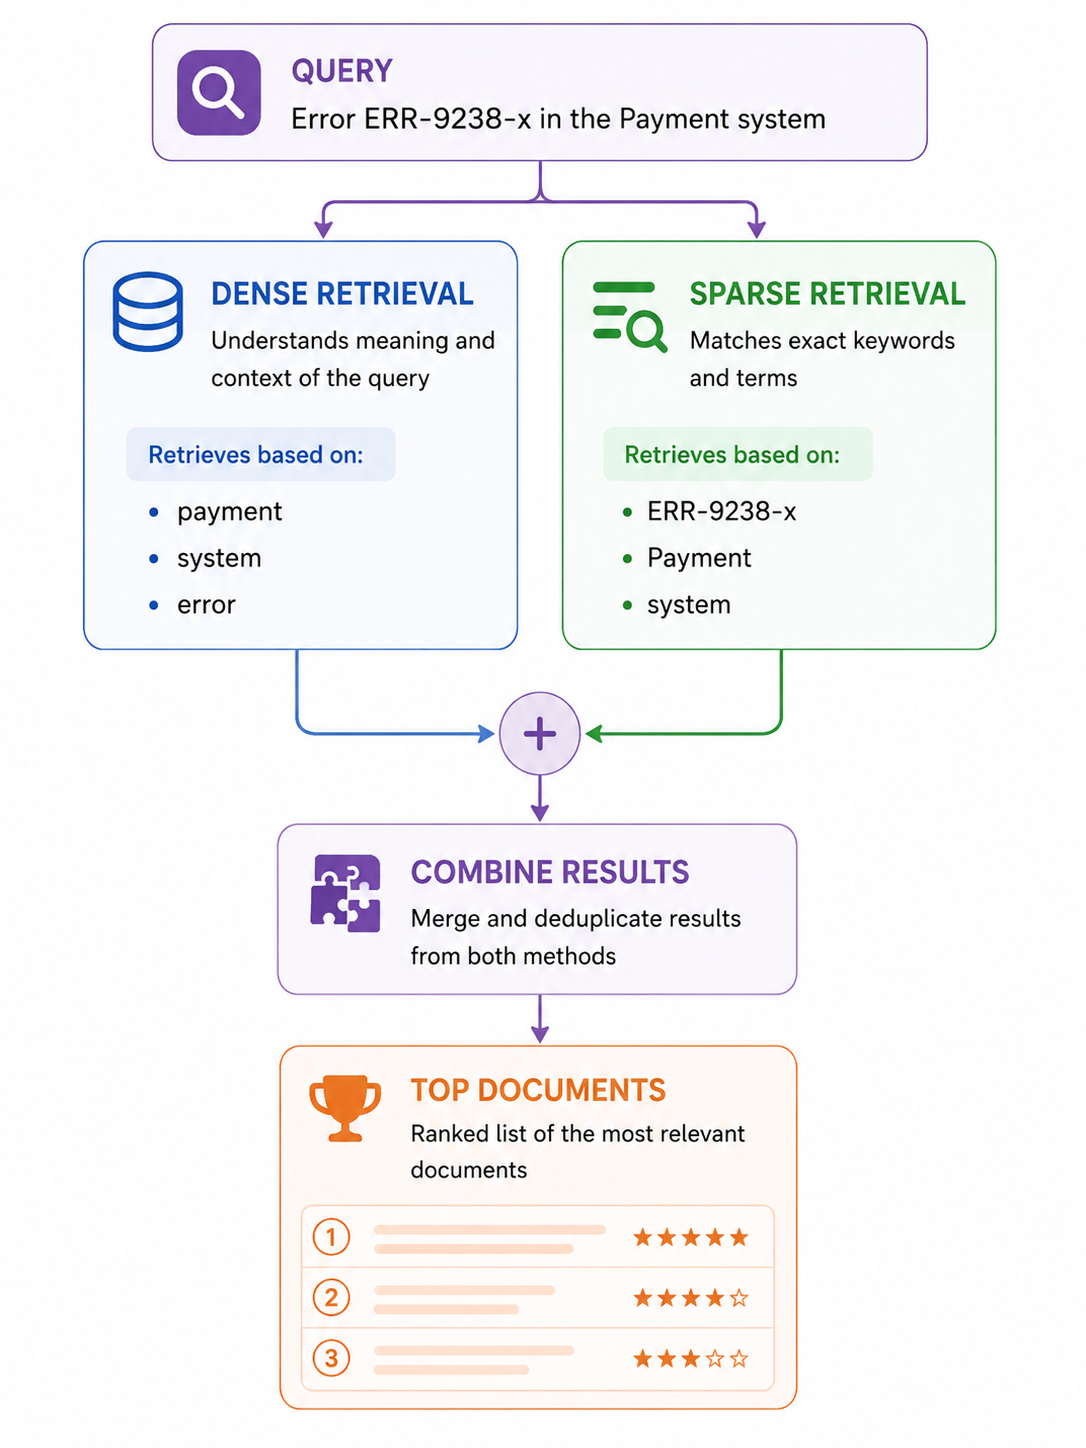
\includegraphics[width=0.85\textwidth]{figures/13-7 figure.png}
\caption{Hybrid search combines dense and sparse retrieval to improve retrieval accuracy.}
\label{fig:hybrid_search}
\end{figure}
\section{Reciprocal Rank Fusion (RRF)}

After performing dense and sparse retrieval, two ranked lists of documents are obtained.

For example,

\begin{center}
Dense:\hspace{0.5cm} A \hspace{0.4cm} B \hspace{0.4cm} C

\vspace{0.2cm}

Sparse:\hspace{0.3cm} B \hspace{0.4cm} D \hspace{0.4cm} A
\end{center}

The challenge is to merge these rankings into a single final ranking.

The most widely used solution is \textbf{Reciprocal Rank Fusion (RRF)}.

Rather than choosing between dense and sparse retrieval, RRF combines their rankings by assigning higher scores to documents that appear near the top of either list.

Consequently,

\begin{itemize}
    \item Dense retrieval contributes semantic understanding.
    \item Sparse retrieval contributes exact keyword matching.
\end{itemize}

By combining both rankings, RRF significantly improves retrieval robustness and accuracy.
\begin{figure}[H]
\centering
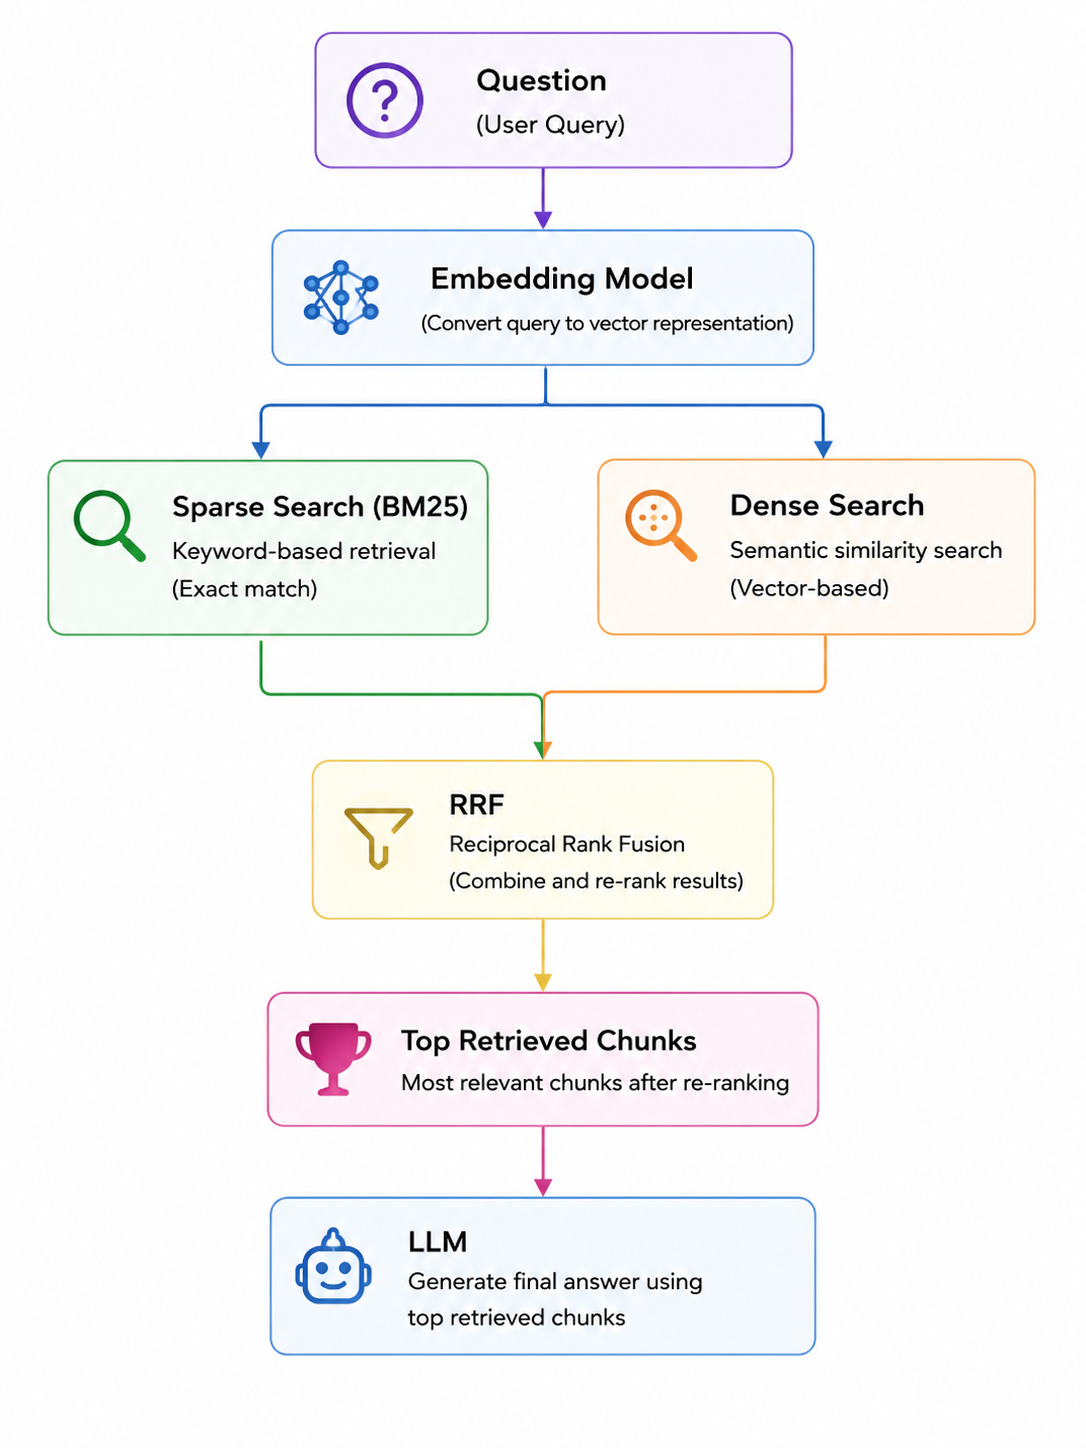
\includegraphics[width=0.85\textwidth]{figures/13-8 figure.png}
\end{figure}
\section{Re-Ranking}

Although the retriever is extremely fast, its ranking is not always optimal.

Assume that the retriever searches thousands of documents and returns the following Top-3 candidates:

\begin{center}
1.\; Chunk A

2.\; Chunk B

3.\; Chunk C
\end{center}

The correct answer may actually be Chunk C rather than Chunk A.

To improve the ranking, a second stage called \textbf{re-ranking} is applied.

Instead of examining every document in the database, the re-ranker only evaluates the retrieved Top-$k$ candidates.

For example, after re-ranking:

\begin{center}
1.\; Chunk C

2.\; Chunk A

3.\; Chunk B
\end{center}

The language model then receives Chunk C, which is the most relevant document.



Many production RAG systems employ hybrid search together with re-ranking because this combination consistently improves retrieval quality.
\begin{figure}[H]
\centering
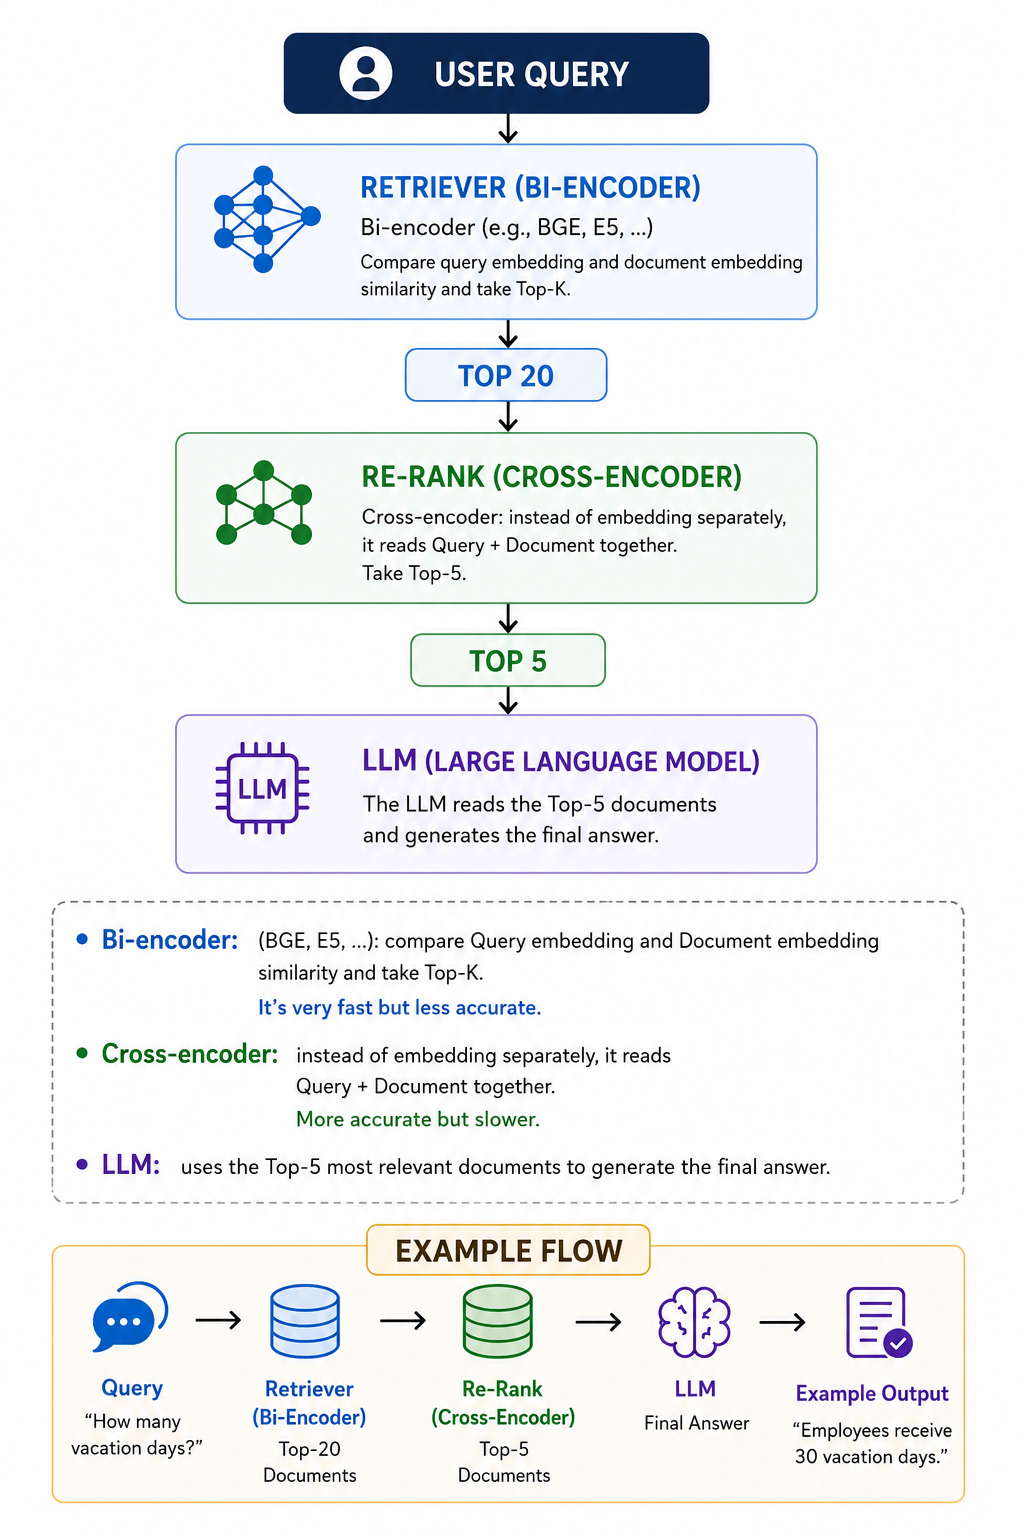
\includegraphics[width=0.85\textwidth]{figures/13-9 figure.png}
\caption{Bi-Encoder retrieval followed by Cross-Encoder re-ranking.}
\label{fig:biencoder_crossencoder}
\end{figure}

Cross-Encoders achieve significantly higher retrieval accuracy because the query and the candidate document are processed together, allowing the model to capture fine-grained interactions between them.

However, this approach is computationally expensive and therefore unsuitable for searching millions of documents directly.

Instead, production RAG systems typically use a two-stage retrieval pipeline:

\begin{enumerate}
    \item A \textbf{Bi-Encoder} efficiently retrieves the Top-$k$ candidate documents from the vector database.
    \item A \textbf{Cross-Encoder} re-ranks only these Top-$k$ candidates to identify the most relevant documents.
\end{enumerate}

This architecture combines the speed of Bi-Encoders with the superior ranking accuracy of Cross-Encoders, making it a common two-stage design used in many production RAG systems.


Modern Retrieval-Augmented Generation (RAG) systems incorporate several additional techniques to improve retrieval quality, reduce computational cost, and provide more accurate responses. These techniques optimize different stages of the retrieval pipeline, including query formulation, document retrieval, context construction, and prompt generation. Together, they significantly enhance the overall performance and robustness of production RAG systems.

\section{Query Optimization}

The quality of retrieval depends heavily on the quality of the user's query. Before searching the knowledge base, many RAG systems optimize the query to improve retrieval accuracy.

\subsection*{Query Rewriting}

A user query is often short, ambiguous, or incomplete. Query rewriting transforms the original query into a clearer and more informative version.

For example,

\begin{quote}
\textbf{Original Query:} Vacation

\textbf{Rewritten Query:} What is the employee vacation policy?
\end{quote}

A better query usually leads to better retrieval because it provides more semantic information to the retriever.

\subsection*{Multi-Query Search}

Instead of performing a single search, the language model generates several alternative versions of the same question.

For example,

\begin{center}
\begin{tabular}{l}
Original Query: \textbf{How many vacation days do employees receive?} \\
\\
Query 1 $\rightarrow$ Annual leave policy \\
Query 2 $\rightarrow$ Employee vacation days \\
Query 3 $\rightarrow$ Paid time off policy
\end{tabular}
\end{center}

Each query is searched independently, and the retrieved results are merged.

This strategy increases \textbf{recall} because different documents may describe the same concept using different wording.
\section{HyDE (Hypothetical Document Embeddings)}

HyDE is an advanced retrieval technique that improves search by generating a hypothetical answer before retrieval.

Instead of embedding the user's question directly, the language model first generates a hypothetical document that is likely to answer the question.

For example,

\begin{quote}
Question: \textbf{What is the vacation policy?}
\end{quote}

The language model may generate the following hypothetical document:

\begin{quote}
``The company grants employees 30 vacation days annually according to the employee handbook.''
\end{quote}

Rather than embedding the original question, the embedding model converts this generated document into a vector.

Because the generated text resembles the type of document stored in the knowledge base, retrieval is often more accurate than embedding the short user query alone.
\section{Context Optimization}

After retrieval, the system has obtained several relevant document chunks. However, sending every retrieved chunk to the language model is not always the best strategy.

Before constructing the final prompt, many RAG systems optimize the retrieved context.

The most common optimization techniques are described below.

\subsection*{1. Duplicate Removal}

Retrieval may return multiple chunks that contain nearly identical information.

Removing duplicate chunks reduces unnecessary tokens while preserving the same knowledge.

\subsection*{2. Context Compression}

Retrieved chunks often contain information that is unrelated to the user's question.

Context compression removes unnecessary sentences while preserving the important information.

This reduces:

\begin{itemize}
    \item Token usage.
    \item Inference cost.
    \item Response latency.
\end{itemize}

\subsection*{3. Lost-in-the-Middle Problem}

Large Language Models tend to pay greater attention to information located at the beginning and the end of the context window.

Consequently, an important chunk placed in the middle of a long prompt may receive less attention.

A common solution is to reorder the retrieved chunks using a re-ranking model so that the most relevant chunks appear first.

\subsection*{4. Dynamic Context Selection}

Instead of always sending a fixed number of retrieved chunks (for example, Top-10), many production systems dynamically choose how many chunks to include.

One common strategy is a score threshold.

For example,

\[
\text{Keep all chunks with similarity score } > 0.8
\]

This approach includes only highly relevant chunks while reducing unnecessary context.
\section{Parent Document Retriever}

Small chunks improve retrieval precision because they contain focused information. However, they often lack sufficient context for the language model.

Conversely, large documents provide rich context but are more difficult to retrieve accurately.

The Parent Document Retriever combines the advantages of both approaches.

Consider the following document:

\begin{itemize}
    \item Page 1: Company Introduction
    \item Page 2: Vacation Policy
    \item Page 3: Vacation Exceptions
    \item Page 4: Vacation Examples
\end{itemize}

Suppose the user asks:

\begin{quote}
\textbf{What is the vacation policy?}
\end{quote}

The retriever correctly identifies the chunk located on Page 2.

If only this chunk is provided to the language model, the model cannot access the exceptions described on Page 3 or the examples presented on Page 4.

To solve this problem, each chunk stores a reference to its parent document.

The indexing process is illustrated below:
\clearpage
\begin{center}
Original Document

$\downarrow$

Split into Small Chunks

$\downarrow$

Each Chunk Stores

\begin{itemize}
    \item Its embedding.
    \item A Parent Document ID.
\end{itemize}
\end{center}

For example,

\begin{center}
\begin{tabular}{ll}
Chunk A & Parent Document 1 \\
Chunk B & Parent Document 2 \\
Chunk C & Parent Document 3 \\
Chunk D & Parent Document 4 \\
\end{tabular}
\end{center}

During retrieval, the following steps are performed:

\begin{enumerate}
    \item Search the vector database using embeddings.
    \item Retrieve the most relevant chunk.
    \item Read its Parent Document ID.
    \item Return the parent document or a larger parent section.
\end{enumerate}

For example, consider a 50-page PDF.

\begin{figure}[H]
\centering
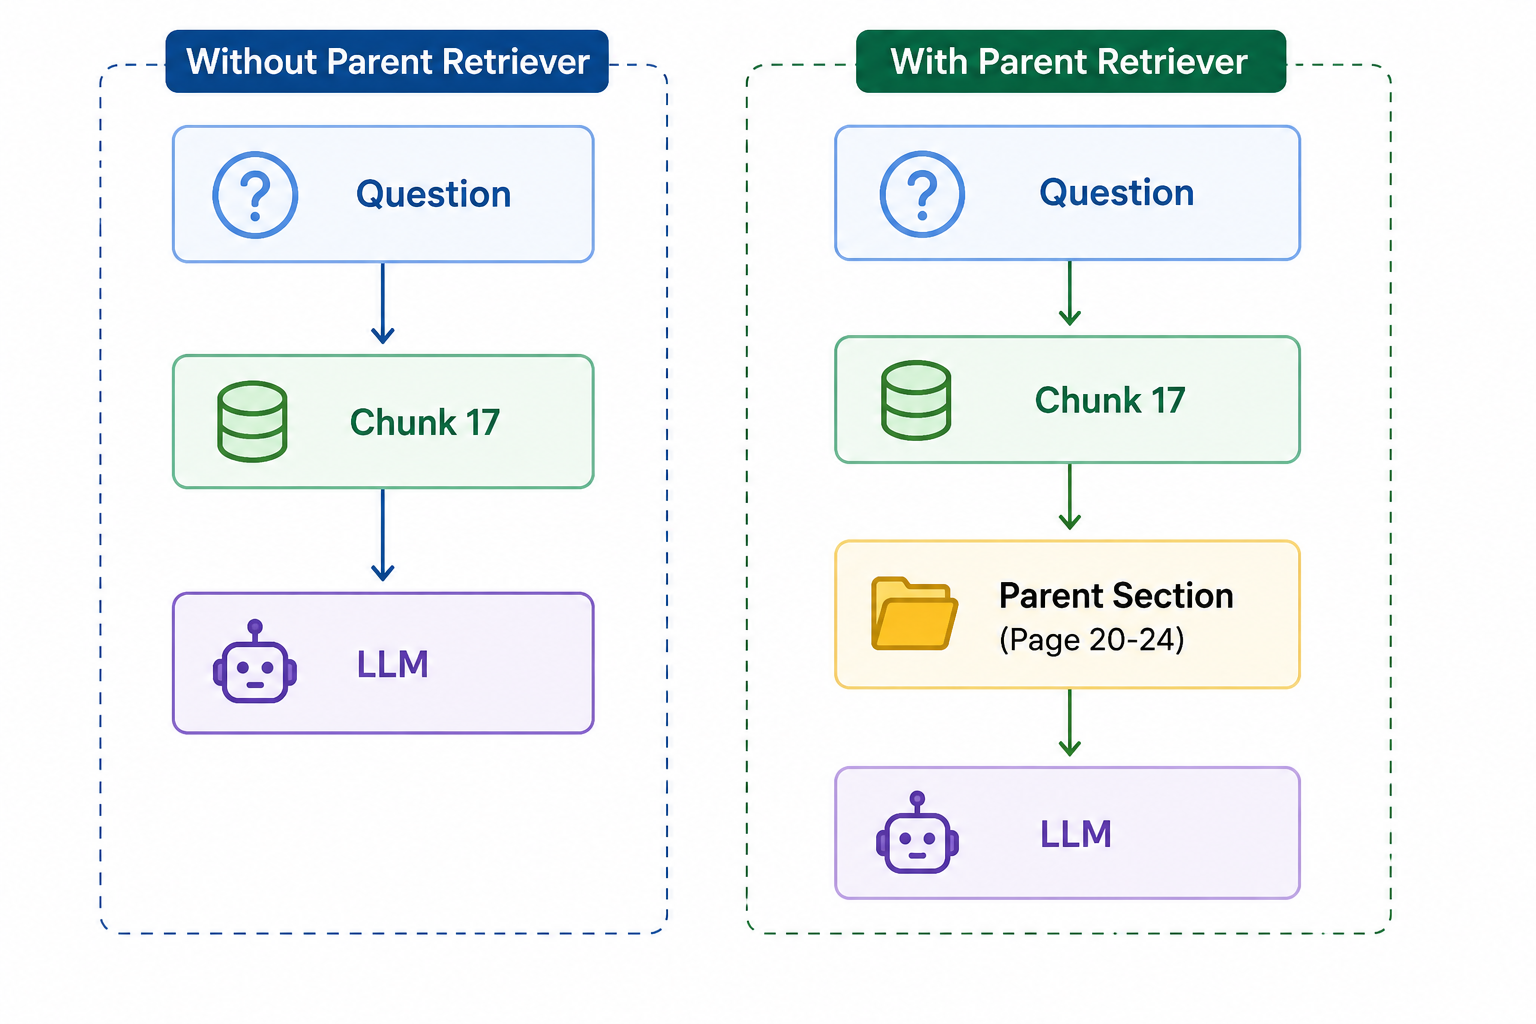
\includegraphics[width=0.85\textwidth]{figures/13-10 figure.png}
\caption{Parent Document Retriever retrieves a relevant chunk and then returns its larger parent document to provide additional context.}
\label{fig:parent_document}
\end{figure}

The Parent Document Retriever is particularly useful for:

\begin{itemize}
    \item PDF manuals.
    \item Books.
    \item Legal documents.
    \item Research papers.
\end{itemize}


\section{Agentic RAG}

Classical Retrieval-Augmented Generation (RAG) follows a fixed retrieval pipeline:

\begin{center}
\textbf{Question $\rightarrow$ Retrieve Once $\rightarrow$ LLM $\rightarrow$ Answer}
\end{center}

This approach works well for simple questions that can be answered using a single retrieval. However, many real-world questions require multiple retrieval steps and intermediate reasoning.

\subsection*{Why Classical RAG Fails}

Consider the following question:

\begin{quote}
\textbf{Which NVIDIA GPU released after the RTX 4090 has more VRAM than the RTX 4080?}
\end{quote}

A single retrieval is usually insufficient because the system must perform several reasoning steps:

\begin{enumerate}
    \item Retrieve the specifications of the RTX 4090.
    \item Retrieve the specifications of the RTX 4080.
    \item Identify NVIDIA GPUs released after the RTX 4090.
    \item Compare their VRAM capacities.
    \item Generate the final answer.
\end{enumerate}

This illustrates that complex questions often require multiple retrieval operations rather than a single search.

\begin{figure}[H]
\centering
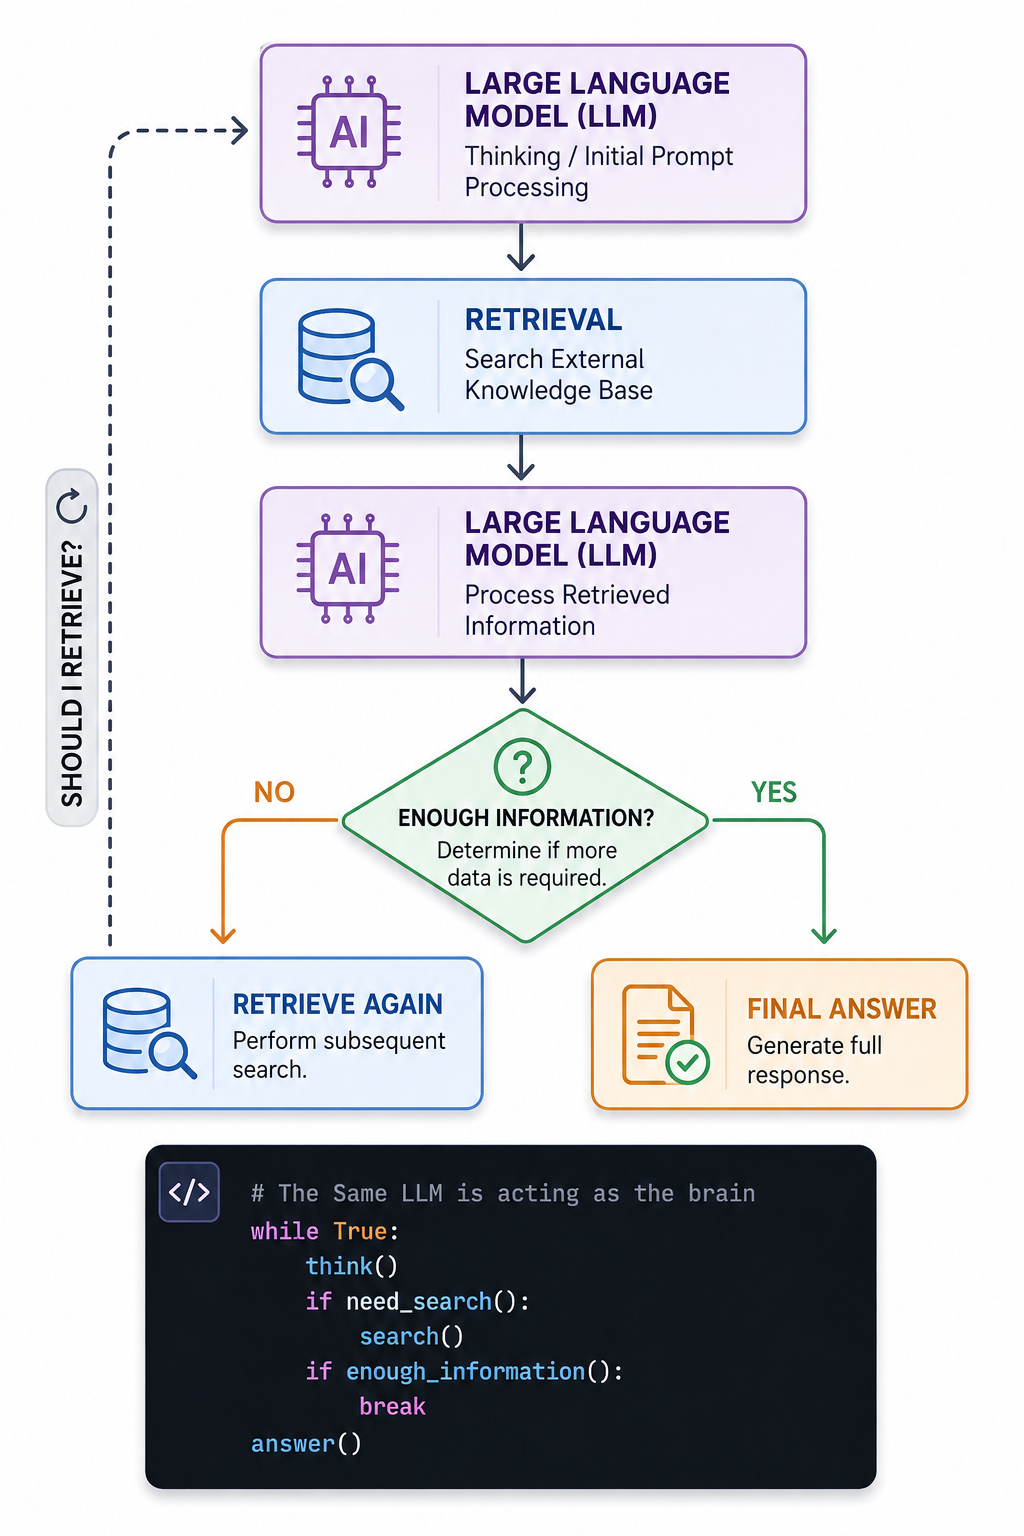
\includegraphics[width=0.85\textwidth]{figures/13-11 figure.png}
\caption{Complex questions often require multiple retrieval and reasoning steps.}
\label{fig:classical_vs_agentic}
\end{figure}

\subsection*{How Agentic RAG Works}

Agentic RAG extends the traditional RAG pipeline by allowing the language model to reason, plan, make decisions, and interact with multiple retrieval tools instead of following a fixed retrieval workflow.

Rather than assuming that one search is sufficient, the language model first analyzes the user's question and determines what information is required.

For simple questions, a single retrieval may be enough.

For more complex questions, the model creates a retrieval plan by decomposing the problem into smaller sub-problems that can be solved sequentially.

For example, consider the following question:

\begin{quote}
\textbf{Which employee manages the department that hired John?}
\end{quote}

The answer cannot be obtained using a single search.

Instead, the agent performs several dependent retrievals:

\begin{enumerate}
    \item Retrieve information about John.
    \item Retrieve information about John's department.
    \item Retrieve information about the department manager.
    \item Generate the final answer.
\end{enumerate}

Each retrieval depends on the result of the previous step, allowing the system to progressively gather the information required to answer the original question.

\subsection*{Dynamic Tool Selection}

During execution, the agent is not restricted to a single retrieval source.

Instead, it dynamically selects the most appropriate tool for each sub-task.

Possible tools include:

\begin{itemize}
    \item Vector databases for document retrieval.
    \item SQL databases for structured information.
    \item External APIs for live data.
    \item Web search engines for external knowledge.
\end{itemize}

The retrieval strategy is therefore adapted dynamically according to the information required at each stage of the reasoning process.

\subsection*{Iterative Retrieval}

After each retrieval, the language model evaluates whether the returned information is sufficient.

If the retrieved documents are incomplete or irrelevant, the agent does not immediately generate an answer.

Instead, it may:

\begin{itemize}
    \item Rewrite the query.
    \item Select another retrieval tool.
    \item Perform an additional search.
\end{itemize}

This iterative process continues until the model determines that it has collected enough reliable information to answer the user's question.

\subsection*{Summary}

Agentic RAG replaces the traditional

\begin{center}
Retrieve Once $\rightarrow$ Answer
\end{center}

pipeline with a dynamic reasoning loop in which the language model:

\begin{itemize}
    \item Plans the retrieval strategy.
    \item Performs one or more retrieval operations.
    \item Chooses the most appropriate retrieval tools.
    \item Evaluates the retrieved information.
    \item Corrects unsuccessful searches when necessary.
    \item Generates the final answer.
\end{itemize}

This reasoning capability makes Agentic RAG significantly more powerful than classical RAG for complex multi-step questions.

\begin{figure}[H]
\centering
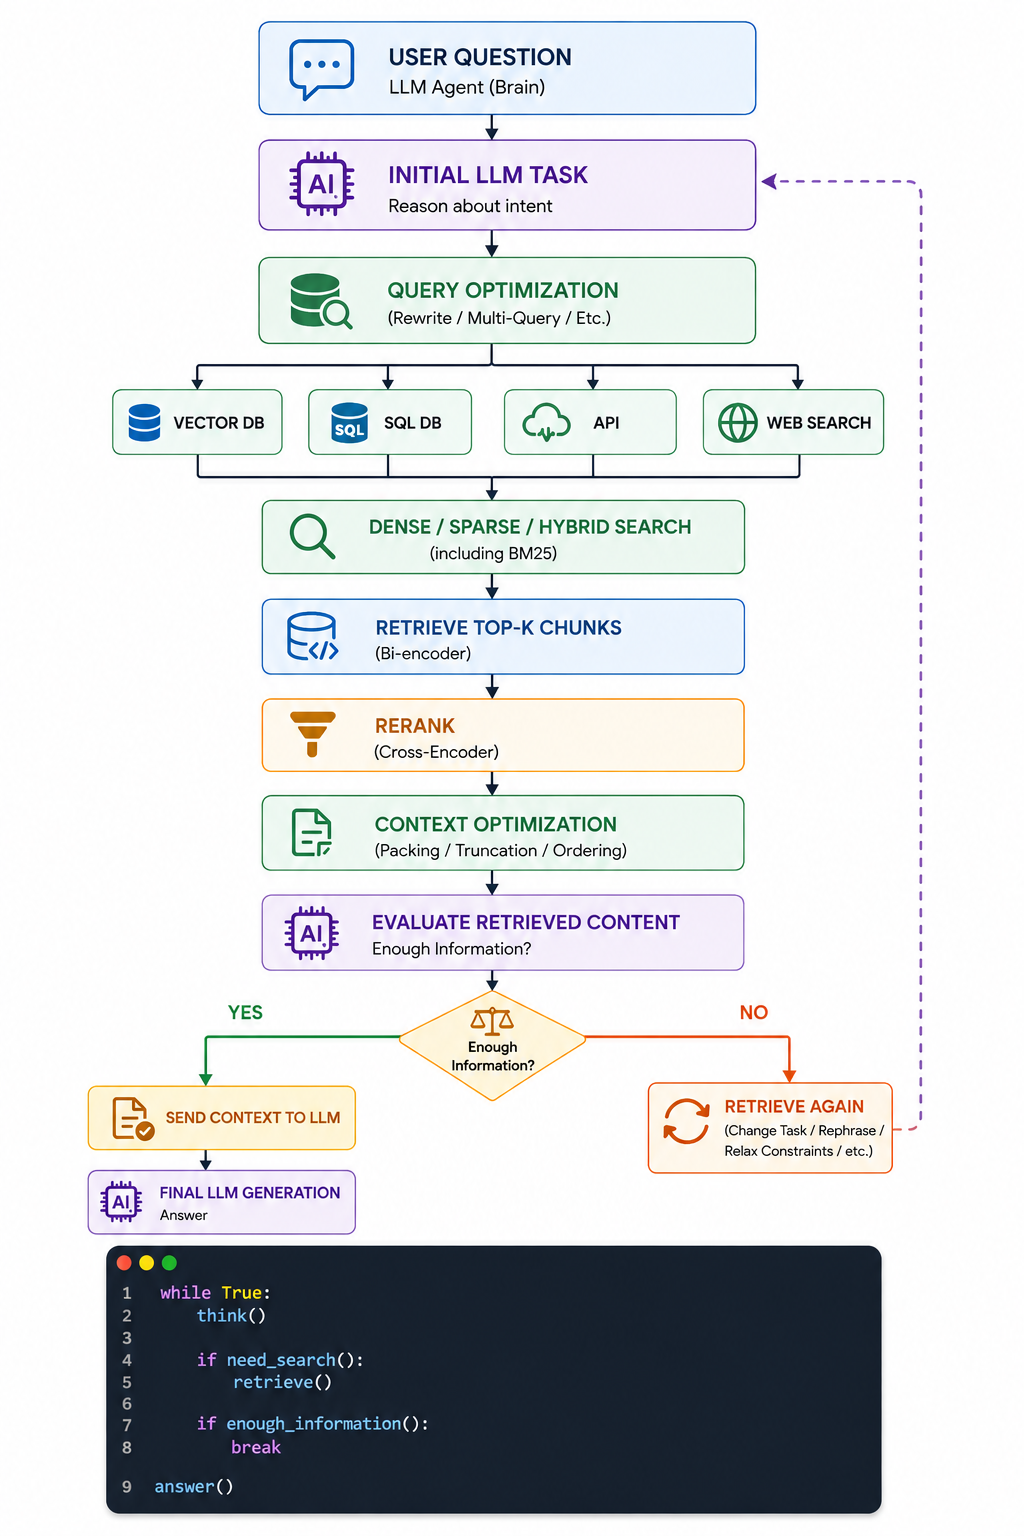
\includegraphics[width=0.85\textwidth]{figures/13-12 figure.png}
\caption{General workflow of an Agentic RAG system.}
\label{fig:agentic_rag}
\end{figure}
\section{RAG Evaluation}

Evaluating a Retrieval-Augmented Generation system requires measuring not only the quality of the generated answer but also the quality of the retrieved information.

The most common evaluation metrics are:

\begin{itemize}
    \item \textbf{Faithfulness}: Is the generated answer supported by the retrieved documents?
    \item \textbf{Groundedness}: Does the answer remain consistent with the retrieved context?
    \item \textbf{Hallucination}: Has the model generated information that is not supported by the retrieved documents?
    \item \textbf{RAGAS}: A popular evaluation framework specifically designed for Retrieval-Augmented Generation systems.
\end{itemize}
\section{Production RAG Systems}

Production RAG systems must remain accurate, efficient, and scalable while the underlying knowledge continuously evolves.

\subsection*{Updating Documents}

Unlike fine-tuning, updating a RAG system does not require retraining the language model.

Suppose the company updates its vacation policy:

\begin{center}
30 Days $\rightarrow$ 35 Days
\end{center}

The update process consists of:

\begin{enumerate}
    \item Updating the document.
    \item Re-chunking the modified content.
    \item Generating new embeddings.
    \item Updating the vector database.
\end{enumerate}

Only the affected document needs to be reprocessed, making updates significantly faster and less expensive than retraining an LLM.

\subsection*{Caching}

Many users often submit identical or very similar questions.

For example,

\begin{quote}
\textbf{What is the vacation policy?}
\end{quote}

Instead of executing the entire retrieval pipeline each time, production systems cache previous retrieval results.

The workflow becomes:

\begin{center}
Question $\rightarrow$ Cache?

Yes $\rightarrow$ Return Cached Result

No $\rightarrow$ Execute the RAG Pipeline
\end{center}

Caching significantly reduces both response latency and computational cost.

\subsection*{Metadata Filtering}

Each chunk stored in the vector database contains metadata that can be used to restrict the search.

For example,

\begin{itemize}
    \item Department = HR
    \item Year = 2025
    \item Language = English
\end{itemize}

Given the query

\begin{quote}
\textbf{Show HR policies from 2025.}
\end{quote}

the retriever searches only documents whose metadata satisfy these constraints, thereby improving retrieval precision.

\subsection*{Scalability}

As the amount of data increases, production systems must continue providing fast responses.

For example,

\[
1000
\rightarrow
10\,000\,000
\rightarrow
1\,000\,000\,000
\]

stored document chunks.

To maintain efficient retrieval, modern systems employ several techniques:

\begin{itemize}
    \item Distributed vector databases.
    \item Approximate Nearest Neighbor (ANN) indexing algorithms such as HNSW and IVF.
    \item Distributed storage of embeddings across multiple machines.
\end{itemize}

These techniques enable production RAG systems to retrieve relevant information within seconds even when billions of document chunks are stored.

A production RAG system is considered scalable when it maintains low latency and high retrieval quality as both the number of stored documents and the number of concurrent users continue to increase.



\section{Monitoring}

Deploying a Retrieval-Augmented Generation (RAG) system is only the beginning. To ensure that the system remains reliable, accurate, and efficient over time, its performance must be continuously monitored.

Monitoring helps detect performance degradation, identify bottlenecks, and improve the overall user experience.

\subsection*{Retrieval Latency}

Retrieval latency measures the time required for the retriever to search the knowledge base and return the relevant document chunks.

For example,

\begin{center}
User Question $\rightarrow$ Retriever $\rightarrow$ 0.08 seconds
\end{center}

If retrieval latency suddenly increases from 0.08 seconds to 3.5 seconds, this indicates that a problem has occurred, such as an overloaded vector database or inefficient indexing.

\subsection*{LLM Latency}

LLM latency measures the time required by the language model to generate the final response.

For example,

\begin{center}
Retriever: 0.1 s

LLM: 8 s
\end{center}

In this case, the language model is the system bottleneck rather than the retriever.

Monitoring each component separately makes it easier to identify where performance improvements are needed.

\subsection*{Hallucination Rate}

Hallucination rate measures how frequently the language model generates information that is not supported by the retrieved documents.

For example, if 100 generated answers are evaluated and

\begin{itemize}
    \item 95 answers are correct,
    \item 5 answers contain hallucinations,
\end{itemize}

then the hallucination rate is

\[
\frac{5}{100}\times100 = 5\%.
\]

If this value later increases to 20\%, it indicates that the quality of the RAG system has degraded and requires investigation.

\subsection*{Failed Queries}

Failed queries are user questions for which the system cannot produce a satisfactory answer.

Typical responses include:

\begin{itemize}
    \item "I don't know."
    \item "No relevant documents found."
    \item "Insufficient information to answer the question."
\end{itemize}

Analyzing failed queries helps identify missing documents, weaknesses in the retrieval pipeline, and information that users frequently search for but cannot currently access.

Monitoring these metrics enables continuous improvement of both the retrieval system and the language model, ensuring that the RAG system remains accurate, efficient, and reliable in production environments.

\section{Advantages and Limitations of RAG}

Retrieval-Augmented Generation provides an effective way to connect Large Language Models with external and continuously changing knowledge. However, RAG is not a universal solution and introduces its own challenges.

\subsection*{Advantages of RAG}

\begin{itemize}

    \item \textbf{Access to External Knowledge:}
    RAG allows an LLM to use information that is not contained in its parameters, including private documents, databases, and internal knowledge bases.

    \item \textbf{Up-to-Date Information:}
    External documents can be updated without retraining the language model. This makes RAG suitable for applications where information changes frequently.

    \item \textbf{Reduced Need for Fine-Tuning:}
    New knowledge can be added to the retrieval system without modifying the model's parameters, significantly reducing training costs.

    \item \textbf{Grounded Responses:}
    The LLM can generate answers based on retrieved documents rather than relying entirely on its internal knowledge, which can help reduce hallucinations.

    \item \textbf{Private and Domain-Specific Knowledge:}
    Organizations can connect an LLM to internal documents and knowledge bases without incorporating all of this information into the model's parameters.

    \item \textbf{Flexible Knowledge Sources:}
    RAG can retrieve information from many different sources, including PDFs, databases, websites, APIs, wikis, and enterprise knowledge bases.

    \item \textbf{Scalability:}
    Large collections of documents can be indexed and searched without increasing the size of the language model itself.

    \item \textbf{Traceability:}
    Retrieved documents can be used to identify the sources that support a generated answer, making the system easier to inspect and evaluate.

\end{itemize}

\subsection*{Limitations of RAG}

Despite its advantages, RAG introduces several challenges that must be addressed carefully.

\begin{itemize}

    \item \textbf{Retrieval Errors:}
    If the relevant document is not retrieved, the LLM may still produce an incorrect or incomplete answer.

    \item \textbf{Poor Chunking:}
    Incorrect chunk sizes or boundaries can separate important information and reduce retrieval quality.

    \item \textbf{Embedding Quality:}
    Poor embeddings may place semantically related documents far apart, causing relevant information to be missed.

    \item \textbf{Context Limitations:}
    Retrieving too many documents can increase the prompt size, cost, and latency while potentially distracting the language model.

    \item \textbf{Additional Infrastructure:}
    A RAG system requires additional components such as document processing pipelines, embedding models, vector databases, and retrieval systems.

    \item \textbf{Latency:}
    Retrieval, re-ranking, context processing, and generation introduce additional processing time compared with a model that answers directly from its parameters.

    \item \textbf{Data Quality:}
    Incorrect, outdated, or contradictory documents can lead to incorrect answers even when the retrieval system works correctly.

    \item \textbf{Complexity:}
    Advanced RAG systems may require query optimization, hybrid retrieval, re-ranking, caching, monitoring, and multiple retrieval tools, making the overall architecture more complex.

\end{itemize}

\subsection*{When Should We Use RAG?}

RAG is particularly useful when an application needs to work with knowledge that is:

\begin{itemize}
    \item Frequently updated.
    \item Private or organization-specific.
    \item Too large to include directly in a prompt.
    \item Stored in external documents or databases.
    \item Required to provide grounded and verifiable answers.
\end{itemize}

RAG is less useful when the required knowledge is stable, general, and already well represented by the model's pretrained knowledge.

The key principle is therefore:

\begin{quote}
\centering
\textbf{Use the model's parameters for general knowledge,}\\
\textbf{and use retrieval for knowledge that changes or lives outside the model.}
\end{quote}
